%************************************************
\chapter{Simulation of Functional Brain Images}\label{ch:simulation}
%************************************************
\section{Simulation Procedure}

\begin{figure}[htp]
	\centering
	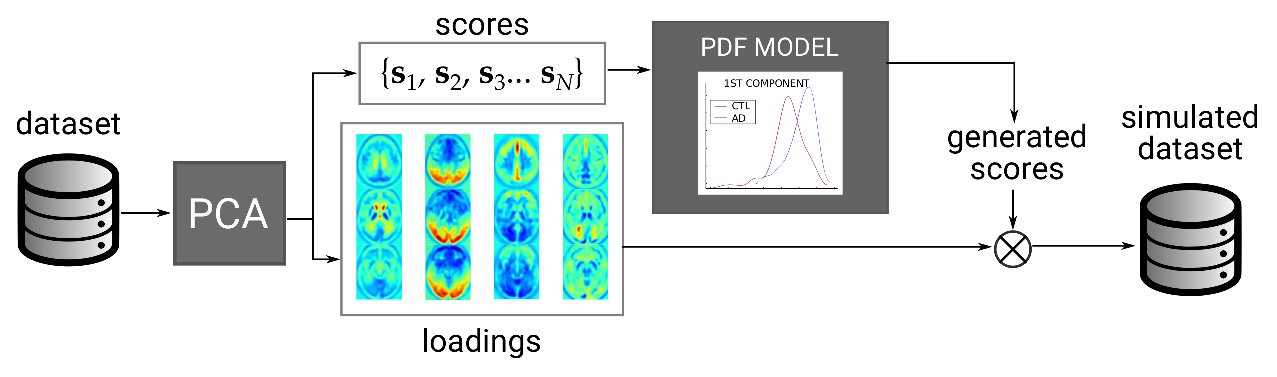
\includegraphics[width=\textwidth]{Graphics/ch9/SchemaGeneration}
	\caption{Schema of the brain image synthesis algorithm.}
	\label{fig:simulationSchema}
\end{figure}
\subsection{Decomposition via PCA}
The first step in our simulation algorithm is to project the original dataset to a new space defined by the principal components of the set; that is, the eigenbrain space. In this space, each subject from the original dataset is projected to a point, and we can afterwards use the space basis (the principal components) to reconstruct that particular subject.in this work we will use the first $N$ components for performance, where $N$ is the number of subjects that are used in the computation of \ac{PCA}. For more details about \ac{PCA}, see Section~\ref{sec:pca}. 

\begin{figure*}[!h]
	\centering
	\includegraphics[width=0.7\linewidth]{Graphics/ch9/originalNOR}\\
	\includegraphics[width=0.7\linewidth]{Graphics/ch9/originalAD}\\
	\includegraphics[width=0.7\linewidth]{Graphics/ch9/generatedNOR}\\
	\includegraphics[width=0.7\linewidth]{Graphics/ch9/generatedAD}
	\caption[Comparison between simulated and original images from \acs{AD} and \acs{CTL} classes.]{Comparison between simulated and original images from \ac{AD} and \ac{CTL} classes.}
	\label{fig:comparisonSimulation}
\end{figure*}

\subsection{Probability Density Modelling using Kernel Density Estimation}
\ac{KDE} is used here to model the statistical distribution of the projected subjects in the eigenbrain space, and it is applied independently to each \ac{AD}, \ac{MCI} and \ac{CTL} class. The \ac{KDE} estimates the probability density function $f$ from a number of independent and identically distributed samples $(x_1, x_2, \dots x_n)$, in the following manner:
\begin{equation}
\hat{f}_h(x) = \frac{1}{n}\sum_{i=1}^n K_h (x - x_i) = \frac{1}{nh} \sum_{i=1}^n K\Big(\frac{x-x_i}{h}\Big),
\end{equation}
where $h>0$ is the bandwidth, a smoothing parameter. The \ac{KDE} via diffusion \cite{Botev2010} used in this article uses a data-driven automatic estimation of the bandwidth, which unlike most methods, does not rely on arbitrary normal reference rules. 

\subsection{Probability Density Modelling using Multivariate Gaussian}

\subsection{Random Number Generation}

\subsection{Brain Image Synthesis}
\section{Experimental Setup}

To validate the simulated dataset, we have performed two different experiments: 
\begin{itemize}
	\item \textbf{Exp. 1}: We have estimated the predictive power of the simulated images by generating new images from the original training set in each cross-validation iteration and using them to predict the original test set. 
	\item \textbf{Exp. 2}: We tested that the simulated images are independent from the original ones, although preserving similar characteristics. To do so, following a Voxel as Features (VAF) approach \cite{Stoeckel04}, we extract a small subset (10 AD and 10 NOR) from the original dataset. Then, we trick the classifier, training it with the whole subset -instead of the training set only-, and testing it against the test set. Therefore, the performance of the tricked system must be close to 1. Then, we generate a new set of simulated images (100 AD and 100 NOR) from the reduced subset and proceed similarly. If our simulated images are independent from the originals, the performance of the system should decrease substantially. 
	
	\end{itemize}
	
	Classification is performed using a Support Vector Machine (SVM) classifier with linear kernel. Estimation of parameter $C$ is performed in an inner cross-validation loop within the training set. Values of accuracy (acc), sensitivity (sens) and specificity (spec) and their standard deviation (SD) are estimated. 
	
\section{Results for ADNI-PET Dataset}

\subsection{Experiment 1}
The performance results for the proposed experiments are shown in Table~\ref{tab:generationResultsExp1}. Exp. 1 is applied to three different scenarios: only AD vs NOR (95 vs 101 subjects), and after incorporating MCI subjects, using them as NOR or AD.  
\begin{table}[h]
	\myfloatalign
	\begin{tabularx}{\textwidth}{cXXX}
		\tableheadline{Scenario} & \tableheadline{acc ($\pm$SD)} & \tableheadline{sens ($\pm$SD)} & \tableheadline{spec ($\pm$SD)}\\
		\midrule
		AD vs NOR & $0.882 \pm 0.012 $ & $0.865 \pm 0.091$ & $0.901 \pm 0.118$\\
		MCI as NOR & $0.727 \pm 0.119 $ & $0.769 \pm 0.155$ & $0.789 \pm 0.151$\\
		MCI as AD & $0.739 \pm 0.126 $ & $0.747 \pm 0.147$ & $0.845 \pm 0.146$\\
		\bottomrule
	\end{tabularx}
	\caption{Baseline performance of the set, using the original dataset.}
	\label{tab:generationResultsExp1}
\end{table}
		
		
\begin{table}[h]
	\myfloatalign
	\begin{tabularx}{\textwidth}{cXXX}
		\tableheadline{Scenario} & \tableheadline{acc ($\pm$SD)} & \tableheadline{sens ($\pm$SD)} & \tableheadline{spec ($\pm$SD)}\\
		\midrule
		AD vs NOR & $0.801 \pm 0.095 $ & $0.782 \pm 0.202$ & $0.821 \pm 0.191$\\
		MCI as NOR & $0.751 \pm 0.078 $ & $0.433 \pm 0.201$ & $0.851 \pm 0.262$\\
		MCI as AD & $0.712 \pm 0.048 $ & $0.821 \pm 0.062$ & $0.382 \pm 0.248$\\
		\bottomrule
	\end{tabularx}
	\caption{Performance of Exp 1, demonstrating the predictive ability of the simulated images over the real dataset.}
	\label{tab:generationResultsExp2}
\end{table}

\begin{table}[h]
	\myfloatalign
	\begin{tabularx}{\textwidth}{cXXX}
		\tableheadline{Scenario} & \tableheadline{acc ($\pm$SD)} & \tableheadline{sens ($\pm$SD)} & \tableheadline{spec ($\pm$SD)}\\
		\midrule
Original & $1.000 \pm 0.000 $ & $1.000 \pm 0.000 $ & $1.000 \pm 0.000 $\\
Simulated & $0.839 \pm 0.094 $ & $0.830 \pm 0.228$ & $0.849 \pm 0.206$\\ 
\bottomrule
\end{tabularx}
\caption{Performance of the Exp 3 proves the independence of the simulated images with respect to the originals.}
\label{tab:generationResultsExp3}
\end{table}

\section{Results for DaTSCAN Datasets}